% -*- root: ../AlgebraConmutativa.tex -*-
\chapter{Ejercicios}

Últimamente nos llegan comentarios de gente que dice que "los apuntes están muy bien, pero me daba vergüenza deciros que el ejercicio $X.Y$ estaba mal". Gracias.

Pero si tú te beneficias de estos ejercicios y crees que están mal, por favor háznoslo saber por email o en persona.

El profesor no va a tener ningún reparo en ponernos un 0 en el examen.

\setcounter{section}{-1} % Start counting from 0
\section{Hoja 0}

\begin{problem}
Sea $R$ un anillo. Demuestra que:

\ppart Si $a \in R$ es un divisor de cero, entonces $a$ no puede ser una unidad.
\ppart Si $R$ es finito, entonces todo $r \in R \setminus \set{0}$ es o bien unidad, o bien un divisor de cero
\ppart Si $R$ no es finito, el enunciado anterior no es necesariamente cierto.
\solution

\doneby{Guille}

\spart

Si $a$ es un divisor de cero, entonces $∃b ∈ R$, con $b ≠ 0$ tal que $ab = 0$. Si $a$ fuese una unidad, podríamos multiplicar por su inverso a ambos lados, y tendríamos que $a'ab = a' 0 \implies b = 0$, contradicción.

\spart

Dado un $r ∈ R^*$, consideramos todas las posibles multiplicaciones por $b ∈ R^*$. Si existe algún $b ∈ R^*$ tal que $rb = 1$, entonces $r$ es una unidad. Si, por otra parte, $rb = 0$, entonces $r$ es divisor de cero.

Vamos a demostrar ahora que el último caso ($r$ no es unidad ni divisor de cero) no se puede dar. Dado que $R$ es finito, por el principio del palomar tiene que haber dos multiplicaciones por elementos distintos que repitan resultado, esto es, $∃b,c ∈ R^*$ tales que $rb = rc$ y $b ≠ c$. Sin embargo, simplemente operando tenemos que $rb - rc = 0$, y por la propiedad asociativa $r(b-c) = 0$, por lo que $r$ sí es divisor de cero, contradicción.

\spart

El principio del palomar no nos vale en cuerpos infinitos. Por ejemplo, en $ℤ$ sólo hay dos unidades y no hay divisores de cero.
\end{problem}

\begin{problem}
Encuentra todas las unidades y los divisores de cero en $\ent$, $\ent_n$ y en $\K[x]$ donde $\K$ es un cuerpo. % de ahí las dos patitas que diría Quirós
\solution
\end{problem}

\begin{problem}
{\bf Sobre las unidades en anillos de polinomios}

Sea $R$ un anillo y sea $R[x]$ el anillo de polinomios con coeficientes en $R$.
\ppart Si $R$ es un dominio de integridad demuestra que
\[ \set{\text{Unidades de } R[x]} = \set{\text{Unidades de } R} \]
\ppart Demuestra, dando un contraejemplo, que el enunciado anterior no es cierto si $R$ no es un dominio de integridad.
\solution

\doneby{Guille}

\spart

Un dominio de integridad no tiene divisores de cero, por lo que nunca nos vamos a poder quitar los monomios de $x^n$ y sólo nos van a quedar las unidades de $R$.

Más formalmente, sea $p(x) = a_0 + a_1 x + \dotsb + a_nx^n$ y $q(x) = b_0 + b_1 x + \dotsb + b_mx^m$ unidades, tales que $p(x) q(x) = 1$. Sin embargo, $p(x) q(x)$ va a tener como coeficiente más alto $a_n b_n x^{m+n}$, y si $p$ y $q$ son unidades el coeficiente de $x^{m+n}$ ha de ser cero para $m+n ≥ 1$. Por lo tanto, o bien $m = n = 0$ y ambos polinomios son de grado cero (luego unidades de $R$) o bien $a_n b_n = 0$, que ya hemos dicho que no ocurre por ser $R$ dominio de integridad.

\spart

Tomamos $ℤ_4[x]$ y $p(x) = 2x + 1$, $q(x) = -2x + 1$. Multiplicando, $p(x) · q(x) = -4x^2 +2x -2x + 1 = 1 \mod 4$, por lo que son unidades de $R[x]$ a pesar de no ser polinomios de grado 0.

\end{problem}

\begin{problem}
Demuestra, dando un contraejemplo, que el conjunto de todos los divisores de cero de un anillo, junto con el 0 no forman, en general, un ideal.
\solution

\doneby{Guille}

Tomamos $ℤ_{6}$, que tiene como divisores de cero $\set{2,3,4}$. Sin embargo, no es un grupo con la suma ya que $2 + 3 = 5$, que no es un divisor de cero.


\end{problem}

\begin{problem}
Demuestra, dando un contraejemplo, que el conjunto de todos los elementos de un anillo que no son unidades no forman, en general, un ideal.
\solution
\end{problem}

\begin{problem}
Demuestra que las siguientes afirmaciones son equivalentes:
\ppart $R$ es un dominio de integridad
\ppart el ideal $\zerogen$ es primo en $R$
\ppart el ideal $\zerogen$ es primo minimal en $R$
\solution
\end{problem}

\begin{problem}
Demuestra que las siguientes afirmaciones son equivalentes:
\ppart $R$ es un cuerpo
\ppart $R$ solo tiene dos ideales, $\zerogen$ y $R$
\ppart El único maximal de $R$ es $\zerogen$
\solution
\end{problem}

\begin{problem}
Sea $\K$ un cuerpo finito
\ppart Demuestra que $\K$ es una extensión finita de $\field_p$ con $p = \mop{char} (\K)$. Concluye que $|\K| = p^n$ para algún $n \geq 1$, $n \in \nat$.
\ppart Demuestra que el homomorfismo de Frobenius que eleva cada elemento a la potencia p es un isomorfismo. Concluye que $\K$ es un cuerpo perfecto.
\ppart Demuestra que $\K$ es un cuerpo de descomposición para el polinomio $x^{p^n}-x$.

Sugerencia: observa que $\K^*$ es un grupo multiplicativo con $p^n - 1$ elementos, concluye que todos los elementos de $\K$ son raíces de $x^{p^n}-x$.
\ppart Deduce del apartado anterior que todos los cuerpos con $p^n$ elementos son isomorfos y que para cada natural $n \geq 1$ hay un cuerpo con $p^n$ elementos. Denotamos por $\field_{p^n}$ al único cuerpo salvo isomorfismo con $p^n$ elementos.
\ppart Usa el apartado c) para demostrar que si $n|m$ entonces $\field_{p^n} \subset \field_{p^m}$ y la extensión es de grado $m/n$.
\ppart Si $\field_{p^n} \subset \field_{p^m}$ demuestra que la extensión es simple.

Sugerencia: usa el Teorema del elemento primitivo.
\ppart Concluye que $\K$ es finito, entonces para cada natural $m \geq 1$, existe al menos un polinomio irreducible de grado m.

Sugerencia: usa los dos apartados anteriores.
\solution

\doneby{Guille}

Dado que no sé si esto lo hemos visto en la teoría, definimos la característica de un cuerpo y la extensión finita.

\begin{defn}[Característica\IS de un cuerpo]
Dado un cuerpo $(\K, +, ·)$, definimos su característica como el número de veces que tenemos que sumar la identidad multiplicativa consigo misma para tener la identidad de la suma. Esto es, si un cuerpo tiene $\mop{char} \K = p$, entonces $\underbracket{\one + \one + \dotsb + \one}_{p\text{ sumas}} = \zero$.
\end{defn}

\begin{defn}[Extensión\IS de cuerpos] \citep[Def. I.1]{apuntesGalois}
Dados dos cuerpos $F$ y $E$ tales que $F⊆E$ diremos que $E$ es una extensión de $F$.

Se escribe $F⊆E$ (obviamente) o también $E/F$.
\end{defn}


\begin{defn}[Grado\IS de una extensión] \citep[Def I.3]{apuntesGalois}
Sea $E/F$ una extensión de cuerpos.
El grado de la extensión es la dimensión de $E$ como espacio vectorial sobre $F$, es decir, \[[E:F] = \dim_FE \]
\end{defn}

Diremos que una extensión es una \concept{Extensión\IS finita} cuando su grado es finito.

\spart

Tenemos que demostrar que \K tiene un subanillo isomorfo a $ℤ_p$ (el hecho de que la extensión finita viene gratis por ser \K finito). Si la característica de \K es $p$, eso significa que $\underbracket{\one + \one + \dotsb + \one}_{p\text{ sumas}}= \zero$. Podemos considerar entonces $\gen{\one} = ℤ_p$, que es un cuerpo (trivial) y además es un subcuerpo de \K, ya que lo hemos generado con las sumas de $n$ veces la unidad, que por definición están en \K.

Falta ahora demostrar que $\card\K = p^n$ para algún $n ≥ 1$. Esto lo sacamos de \citep[Ej. 1.4]{apuntesGalois}. Definimos un homorfismo de anillos $φ$ de la siguiente forma: \begin{align*} \appl{φ}{ℤ&}{K} \\
α &\longmapsto α · \one
\end{align*}

Estudiemos el núcleo de φ. Son los elementos de $ℤ$ cuya imagen es la unidad en $\K$, esto es, tomando $n = \mop{char}(\K)$, \[ \ker φ = \set{a·n \tq a ∈ ℤ} = nℤ \]

El segundo teorema de isomorfía de grupos\footnote{Ver magníficos apuntes de Pedro Valero de Estructuras Algebraicas \citep{apuntesEA}.} nos dice que existe un isomorfismo entre la imagen de $φ$ y el grupo cociente $\quot{ℤ}{\ker φ}$, al que llamaremos $γ$:

\[ \appl{γ}{\quot{ℤ}{nℤ}}{\img φ ⊆ \K} \]

Afirmamos que $n≠0$: $\K$ es finito y $\quot{ℤ}{0ℤ} = ℤ$, así que no puede existir un isomorfismo entre ambos.

Afirmamos que $n$ es primo, y vamos a demostrarlo por reducción al absurdo. Supongamos $n = ab$. Si operamos en $\fd_n$, tenemos que $n\equiv 0 \mod n$ y entonces $ab=0$. Aplicamos $γ$ a ambos lados y tendríamos que $γ(a)·γ(b) = γ(0) = 0_\K$, contradicción ($\K$ es un cuerpo así que no puede tener divisores de $0$).

Sea $p=n$, entonces \[ \mathbb{F}_p = \quot{ℤ}{nℤ}  \simeq \img φ \] es un subcuerpo de $\K$, luego $\K$ es un espacio vectorial sobre $\mathbb{F}_p$. Es decir, que si $[\K:\mathbb{F}_p] = m$, entonces $\{x₁, \dotsc, x_m\}$ es base de $\K$ sobre $\mathbb{F}_p$, luego \[ \card{\K} = \card{\fd_p}^{[\K:\fd_p]} = p^m\] para $m ≥ 1$, y ya tenemos lo que buscábamos.

Una observación importante: el cuerpo finito de $n$ elementos \textbf{no es} $\quot{ℤ}{nℤ}$. Los enteros módulo $n$ sólo son un cuerpo cuando $n$ es primo. Es decir, que en general \[ \fd_n ≠ \quot{ℤ}{nℤ} \].

Los cuerpos finitos hay que construirlos específicamente como el cociente de un cuerpo finito de orden primo con el ideal generado por un polinomio irreducible. Por ejemplo, podríamos preguntarnos si hay un cuerpo con 9 elementos. Existe, porque $9=3^2$.

\spart

A modo de nota, por ser $\K$ un cuerpo es un dominio de integridad (no tiene divisores de cero) y por lo tanto si tiene característica $p$, $p$ debe ser primo\footnote{Si tuviésemos que $p$ no es primo, lo podemos descomponer como producto factores primos $p = a_1·a_2\dotsb a_n$ con $a_i ≠ \one$. Entonces $\zero = p · \one = a_1\one · a_2 \one \dotsb a_n \one = \zero$, pero como no tenemos divisores de cero alguno de esos $a_i \one$ debe ser cero, y por lo tanto el cuerpo tiene característica $a_i$, con $a_i$ primo.}.


Denotaremos el \concept{Homomorfismo\IS de Frobenius} como $φ(x) = x^p$. Probamos primero que es compatible con las operaciones. Vemos que \[ φ(a+b) = (a+b)^p = \sum_{n=0}^p \comb{p}{n} a^{p-n} b^n \], sin embargo, salvo para $n = 0$ y $n = p$, los coeficientes serán divisibles por $p$ y por lo tanto serán $0$. Entonces $φ(a+b) = a^p + b^p = φ(a) + φ(b)$, luego φ es compatible con la suma. La compatibilidad con el producto es trivial.

Vamos a comprobar ahora que es biyectivo. Tenemos $a, b ∈ \K$ distintos, y supongamos que $φ(a) = φ(b)$. Entonces, $0 = φ(a) - φ(b) = φ(a-b) = (a-b)^p$. Ahora bien, por ser \K un cuerpo (y sin divisores de cero por lo tanto) sólo puede ser $a-b = 0$, por lo que $a$ y $b$ son iguales, contradicción.

Por último, para que sea sobreyectivo tenemos que ver que para todo $a ∈ \K$ existe un $b ∈ \K$ tal que $φ(b) = a$. La cuestión es que como \K es un cuerpo finito y ya hemos demostrado que φ es inyectivo no queda otra opción: por el principio del palomar, si nos quitamos un elemento de la imagen de $φ$, habría un $c ∈ \K$ que es imagen de dos elementos de \K y entonces φ no sería inyectivo.

La definición de \concept{Cuerpo\IS perfecto} es esta misma: que el homomorfismo de Frobenius es un automorfismo (isomorfismo consigo mismo).

\spart

Por el Teorema de Lagrange, el orden de cualquier elemento de un grupo tiene que dividir al orden del grupo. Dado que $\K^*$ es un grupo con la multiplicación de orden $p^n - 1$, por lo que $∀x ∈ \K^*$ tenemos que $x^{p^n - 1} = \one$. Si operamos, tenemos que \[  x^{p^n - 1} = \one \implies x^{p^n} = x \implies x^{p^n} - x = 0 \]

Por lo tanto, todos los elementos en $\K^*$ son ceros de ese polinomio. Trivialmente vemos que \zero también es cero de ese polinomio, por lo tanto todos los elementos de \K son raíces.

\spart

\K es el cuerpo de descomposición del polinomio $x^{p^n} - x$, y los cuerpos de descomposición existen y son únicos salvo isomorfismo\footnote{Vía Wikipedia, yo me lo creo.}.

\spart

Si $n|m$, podemos decir que $m = kn$ para algún $k ∈ ℕ$. Los elementos de ambos cuerpos $\field_{p^n}$ y $\field_{p^m}$ son raíces de los polinomios $x^{p^n} -x$ y $x^{p^m} - x$ respectivamente. Ahora bien, $p^m = p^{kn} = (p^n)^k$, y por lo tanto $x^{p^m} = x^{(p^n)^k} = x^{p^n · p^n \dotsb p^n} = (((x^{p^n})^{p^n})^{p^n})^{\dotsb} = x$, por lo que todo $x ∈ \field_{p^n}$ es raíz de $\field_{p^m}$ y por lo tanto $x ∈ \field_{p^m}$.

\spart

Primero definimos qué es una extensión simple.

\begin{defn}[Extensión\IS simple] Una extensión de cuerpos $L/K$ es una extensión simple de grado $n$ si existe un elemento primitivo $X ∈ L$ tal que \[ L = K(X) = \set{a + a_1 X + \dotsb + a_{n-1}X^{n-1}\tq a_i ∈ K} \]

Por ejemplo, $ℚ(\sqrt{2})$ son los números de la forma $a + b\sqrt{2}$ y es una extensión simple de $ℚ$.
\end{defn}

\begin{theorem}[Teorema\IS del elemento primitivo] Sea $L/K$ una extensión finita y separable. Entonces, es una extensión simple.
\end{theorem}

Con esto ya tenemos el ejercicio hecho: el apartado anterior nos dice que $\field_{p^n} ⊂ \field_{p^m}$ es una extensión y por ser finita es simple gracias al teorema del elemento primitivo.

\spart

Si $\K = \field_{p^n}$ es finito, entonces siempre podemos encontrar un cuerpo $\field_{p^{nm}}$ cuya extensión sea de grado $\frac{nm}{n} = m$, que por el teorema del elemento primitivo está generada por un elemento $X ∈ \field_{p^{nm}}$. Por ser una extensión de grado $m$, tenemos que $X^m ∈ \field_{p^n}$ (si no, sería una extensión de grado superior). En ese caso, $x^{mn} - X^{m}$ es un polinomio que tiene como raíz $X$ y por lo tanto se nos va a quedar algún factor de grado mayor que uno irreducible en $\field_{p^n}$.

\end{problem}

%%%%%%%%%%%%%%%%%%%%%%%%%%%%%%%%%%%%%%%%%%%%%%%%%%%%%%%%%%%%%%%%%%%%%%%
\section{Hoja 1: Anillos, ideales}

\begin{problem}
{\bfseries El radical de un ideal.}

Sea $I\subset R$ un ideal  y sea $\sqrt{I}$ su radical.

\ppart Demuestra que $\sqrt{I}$ es un ideal que además contiene a $I$.

\ppart Demuestra que todo ideal primo es radical.

\ppart Describe todos los ideales de ${\mathbb Z}$ que sean radicales.

\ppart Sea $\K$ un cuerpo. Describe todos los ideales de $\K[x]$ que sean radicales.

{\em Sugerencia: utiliza el ejercicio 1  de la parte de problemas para entregar.}

\solution

\doneby{Guille}

Recordamos la definición de \nlref{def:RadicalIdeal}: son los elementos del anillo que tienen una potencia en el ideal.

\spart

Primero tenemos que comprobar que el radical está cerrado por la suma. Sean $a,b ∈ \sqrt{I}$ tales que $∃m,n ∈ ℕ$ con $a^m ∈ I,\;b^n ∈ I$. Supongamos, sin pérdida de generalidad, que $m > n$. Queremos ver que $a+b ∈ \sqrt{I}$ o, equivalentemente, que $∃s ∈ ℕ$ tal que $(a+b)^s ∈ I$. Podemos tomar $s = m + n$, de tal forma que el desarrollo en serie de potencias sea \[ (a+b)^s = \sum_{k=0}^{m+n} \comb{m+n}{k} a^{m+n-k}b^k \]

Para $k = 0, \dotsc, m$, tendremos que $a^{m+n-k} = a^m·a^{n-k} ∈ I$ por absorción ($a^m ∈ I$). Cuando $k > m$, tendremos que $b^k ∈ I$ por la misma razón, por lo que siempre tendremos que los elementos de la suma estarán en $I$ y entonces $(a+b)^s ∈ I$.

La propiedad de absorción es considerablemente más sencilla: si $a∈\sqrt{I}$ con $a^m ∈ I$, entonces $∀b ∈ R$ tendremos que $(ba)^m = b^m a^m ∈ I$.

\spart

Un ideal es primo (\fref{def:IdealPrimo}) cuando cada vez que $a · b ∈ I$, se tiene que $a ∈ I$ o $b ∈ I$. Dado que ningún elemento de $I$ sale del producto de elementos de fuera de $I$, podemos escribir $I = \gen{a_1, \dotsc, a_n}$, esto es, $I$ está generado por elementos de $I$ multiplicados por sí mismos o por elementos de $R$. De aquí podemos construir otro ideal $S = \gen{a_1^{m_1}, \dotsc, a_n^{m_n}}$, que seguirá siendo un ideal y del cual $I$ es radical. % Triplazo.

\spart

% No me apetece

\spart

Por una parte, tendremos todos los radicales de $\K$, y $\gen{x}$. \textit{No me apetece pensarlo mucho más, probablemente esté mal.}

\end{problem}

\begin{problem}
{\bfseries Unión de ideales.}

La unión de ideales no siempre es un ideal.

\ppart Sean $I,J\subset R$ dos ideales. Demuestra que, en general, $I\cup J$ no es un ideal.

\ppart  Sea $I_1\subset I_2\subset \ldots \subset I_n \subset \ldots$  una sucesión creciente (no necesariamente finita) de ideales en $R$.
Demuestra que la unión $\cup_{n}I_n$ es un ideal en $R$.

\ppart Demuestra que en ${\mathbb Z}$, $\langle n\rangle +\langle m\rangle=\langle k\rangle$ con $k=\text{gcd}(n,m)$.
\solution
\end{problem}

\begin{problem}
{\bfseries Intersección de ideales.}

La intersección de ideales siempre es un ideal que no hay que confundir con el producto de ideales.

\ppart Sea $\{I_i\}_{i\in {\mathcal I}}$ una colección de ideales.  Demuestra que $\cap_{i\in {\mathcal I}} I_i$ es un ideal en $R$.

\ppart  Demuestra que en ${\mathbb Z}$, $\langle n\rangle \cap \langle m\rangle=\langle k\rangle$ con $k=\text{m.c.m.}(n,m)$.

\ppart  Sean $I, J\subset R$ dos ideales. Demuestra que $I\cdot J\subset I\cap J$; encuentra un ejemplo para el que la inclusión sea estricta.
\solution
\end{problem}

\begin{problem}
{\bfseries ¿Cuándo es la intersección de ideales igual al producto?}

Se dice que dos ideales $I, J\subset R$ son coprimos si $I+J=R$.

\ppart Encuentra dos ideales coprimos en
$Z$, y otros dos en ${\mathbb R}[x,y]$.

\ppart Demuestra que si $I$ y $J$ son coprimos, entonces  $I\cdot J=I\cap J$.

\ppart Sean $I_1,\ldots I_n$ ideales en $R$. Demuestra, usando inducción en $n$, que si los ideales son primos dos a dos entonces $\prod_iI_i=\cap_iI_i$.

\noindent{\em Sugerencia para (a): si $I$ y $J$ son coprimos, entonces existen $x\in I$ e $y\in J$ tales que $x+y=1$;
ahora multiplica la expresión anterior por  $a\in I\cap J$.

Sugerencia para (b): define $J=\prod_{I=1}^{n-1}I_i$; como los ideales $I_i$ son coprimos dos a dos, existen $y_i\in I_n$, y
$x_i\in I_i$, $i=1,\ldots, n-1$, tales que $x_i+y_i=1$; ahora utiliza el producto $\prod_{i=1}^{n-1}x_i$ para probar que
$I_n$ y $J$ son coprimos. }
\solution
\end{problem}

\begin{problem}
{\bfseries La geometría que veremos.}

Sean $I_1,\ldots, I_n$ ideales en $R$, y sea $\mathfrak p \subset R$ un ideal primo que contiene a
$\cap_iI_i$, esto es, $\cap_iI_i\subset \mathfrak p$. Demuestra que:

\ppart $I_i\subset \mathfrak p$ para algún $i\in \{1,\ldots,n\}$;

\ppart Si además  $\cap_iI_i=\mathfrak p$ entonces $I_i=\mathfrak p$ para algún $i\in \{1,\ldots,n\}$.

\noindent{\em {Sugerencia para (a)}: si $ I_i \nsubseteq \mathfrak p$ para $i=1,\ldots,n$ entonces para cada $i$ existe un elemento $b_i\in I_i $ con $b_i\notin \mathfrak p$; ahora considera $\prod_ib_i$. }

\solution

\doneby{Guille}

\spart

Seguimos la sugerencia y demostramos por reducción al absurdo: no existe ningún $I_i$ tal que $I_i ⊆ \mathfrak{p}$. Por lo tanto, para cada $i = 1, \dotsc, n$ existe un $b_i ∈ I_i$ con $b_i ∉ \mathfrak{p}$. Consideramos ahora $\prod b_i$, que podemos expresar como \[ \prod_{i=1}^n b_i = b_k · \prod_{\substack{i = 1 \\ i ≠ k}}^n b_i \eqreasonup[∈]{Absorción} I_k \]

Como tenemos que el producto está en $I_k$ para todo $k$, tenemos que $\prod b_i ∈ \bigcap I_i$ y entonces $\prod b_i ∈ \mathfrak{p}$. Ahora bien, $\mathfrak{p}$ es primo, por lo que si el producto de todos esos elementos está en $\mathfrak{p}$, entonces su producto ha de estar obligatoriamente en $\mathfrak{p}$, contradicción.

\spart

De nuevo por reducción al absurdo. Si $I_i ≠ \mathfrak{p}$, entonces para cada $i = 1, \dotsc, n$ existe un $b_i ∈ I_i$ y (al menos un) $j = 1, \dotsc, n$, $j ≠ i$, con $b_i ∉ I_j$ de tal forma que $b_i ∉ \mathfrak{p}$.

\end{problem}

\begin{problem}
{\bfseries Miramos ejemplos en $\ent$.}

En ${\mathbb Z}$ observa que $\langle 36\rangle \subset \langle 3\rangle$, $\langle 2\rangle$;
encuentra todas las maneras de escribir $\langle 36\rangle$ como intersección de ideales. A la vista del problema anterior,  ¿qué crees que va a suceder?
\solution
\end{problem}

\begin{problem}
{\bfseries Anillos locales.}

Demuestra que las siguientes afirmaciones son equivalentes:

\ppart $R$ es un anillo local con ideal maximal $\mathfrak m$;

\ppart $R$ contiene un ideal  $\mathfrak m$ tal que todo elemento de $R\setminus \mathfrak m$ es una unidad.
\solution
\end{problem}

\begin{problem}
Sea $k$ un cuerpo. Definimos el anillo de series formales en una variable sobre $k$ como el conjunto
$$k[|t|]:=\left\{\sum_{i=0}^{\infty}a_it^i: a_i\in k\right\}$$
con la suma y el producto habituales. Demuestra que $\alpha=\sum_{i=0}^{\infty}a_it^i
  \in k[|t|] $ es una unidad si y sólo si $a_0\neq 0$. Concluye que $k[|t|]$ es un anillo local cuyo único ideal maximal es además  principal.
\solution
\end{problem}

\noindent \fbox{{\bfseries  Problemas para entregar (CORREGIDOS!)} }

\textbf{Pongo las correcciones de Ana en azul}

% --------------------------------------------------- %
% ----------------- PROBLEMA 1.9 -------------------- %
% --------------------------------------------------- %
\begin{problem}
{\bfseries Sobre los ideales en $K[x]$. Sea K un cuerpo}

\ppart Demuestra que $K[x]$ es un dominio euclídeo.
\ppart Demuestra que en $K[x]$ todos los ideales son principales.
\ppart Demuestra que en $K[x]$ un ideal es maximal si y solo si está generado por un polinomio irreducible.
\ppart Demuestra que en $K[x,y]$ no todos los ideales son principales. {\em Sugerencia: considera el conjunto $I$ formado por todos los polinomios $p(x,y)\in K[x,y]$ que se anulan en $(0,0)$; demuestra que es un ideal y que no es principal.}

\solution


\begin{defn} \textbf{Dominio Euclídeo}
	Es un par $(K, \phi)$ donde $K$ es un dominio de integridad y $\phi$ es una aplicación norma euclídea, es decir: $\phi: K \setminus \{0\} \rightarrow \nat$ cumple:
	\begin{enumerate}
		\item Si $a,b \in K \setminus \{0\}$, se cumple que $a | b \implies \phi(a) \leq \phi(b)$
		\item $\forall a,b \in K$, con $b \neq 0$, $\exists q,r \in K$ tal que $a=bq+r$ con $r=0$ ó $\phi(r) < \phi(b)$
	\end{enumerate}
\end{defn}

Para demostrar que $K[x]$ es un dominio euclídeo, tenemos que definir una aplicación $\phi$ que sea norma euclídea.

Sea $\phi$ una aplicación que asigna a cada polinomio su grado, $\phi(p(x)) = \mop{gr} p(x)$. Vamos a probar que $\phi: K[x] \setminus \{0\} \rightarrow \nat$ es una aplicación norma euclídea:
\begin{enumerate}
	\item Si tenemos $p(x) | q(x)$, entonces quiere decir que $q(x)=p(x)\cdot r(x)$, con $r(x) \in K[x] \setminus \{0\}$. Es obvio que el grado de $p(x)$ es menor o igual que el grado de $p(x)\cdot r(x)$.
	\item Sea $a(x), b(x) \in K[x]$, con $b(x) \neq 0$, tenemos que ver que existe $r(x), q(x) \in K[x]$ tal que $a(x)=b(x)q(x)+r(x)$ con $r(x)=0$ ó $\mop{gr} r(x) < \mop{gr} b(x)$.

	Eso también es cierto. Utilizando el algoritmo de la división (\textcolor{blue}{por inducción en el grado de $b$}), existen $q,r \in K[x]$ tales que $c=bq+r$ con $r=0$ ó $\phi(r) < \phi(b)$.
\end{enumerate}

\spart


\begin{defToUse}
	\begin{itemize}
		\item \textbf{Ideal}: Sea $(R,+,\cdot)$ un anillo y sea $I \subseteq R$. Se dice que $I$ es un ideal si:
		\begin{enumerate}
			\item $I \neq \emptyset$
			\item $(I, +)$ es un subgrupo de R.
			\item Propiedad de absorción: $\forall i \in I, \forall r \in R \implies r\cdot i \in I$.
		\end{enumerate}
		\item \textbf{Ideal generado por $T$}: Definimos el ideal generado por $T$ como el ideal más pequeño de $R$ que contiene a $T$ y se denota por $\gen{T}$.

		Explícitamente, sea $R$ un anillo y $T \subset R$ no vacío, entonces:
		$$ \gen{T} = \{r_1t_1+...+r_st_s: r_i \in R, t_i \in T, s \geq 1 \} $$.
		\item \textbf{Ideal principal}: Un ideal es principal si está generado por un único elemento.
	\end{itemize}
\end{defToUse}

Sea $K[x]$ dominio euclídeo, y sea $I$ un ideal de $K[x]$. Por definición, $I$ es subgrupo normal de $K[x]$. Si $I=\set{0}$ es claro que es un ideal principal. Supongamos entonces que $I$ contiene al menos un elemento distinto de 0.

Sea $a \in I$, tal que $\phi(a) \leq \phi(c)$ para cualquier otro $c\in I$. Entonces, utilizando el algoritmo de la división, existen $q,r \in K$ tales que $c=qa+r$ con $r=0$ ó $\phi(r) < \phi(a)$.

Pero $r=c-qa \in I$, $r \neq 0$, implicaría $\phi(r) \geq \phi(a)$, por la definición de $a$, en contra de las hipótesis del algoritmo de la división. Por tanto, tendríamos que tener $r=0$, y todo elemento $c\in I$ es de la forma $c=qa$, por tanto, $I=\gen{a}$.

\spart


\begin{defToUse}
	\nref{def:IdealMaximal}: Un ideal $I \subsetneq R$ es maximal si cualquier otro ideal que lo contenga es o bien él mismo o bien el total.
\end{defToUse}


En el apartado anterior hemos demostrado que todos los ideales son principales, esto es, están generados por un único elemento. Sea $I$ un ideal generado por $p(x) ∈ K[x]$ irreducible. Para que otro ideal $J = \gen{q(x)}$ contenga a $I$, $q(x)$ tiene que dividir a $p(x)$. Sin embargo, por ser $p(x)$ irreducible, $q(x)$ sólo puede ser o bien $q(x)$ (y entonces $J = I$) o bien $1$ (y entonces $J = K[x]$).

Para la implicación al otro lado, vemos que si $\gen{p(x)} = I \subsetneq K[x]$ es maximal, entonces no hay ningún ideal propio que lo contenga. Por lo tanto, si consideramos cualquier otro ideal $J = \gen{q(x)}$ con $q(x) ≠ 1,\,q(x) ≠ p(x)$, tenemos que $I \subset J$ o, equivalentemente, no existe ningún $q(x)$ que divida a $p(x)$ (salvo $1$ y $p(x)$, que ya hemos excluido). Es decir, $p(x)$ es irreducible.

\spart

Este ejercicio se resuelve cogiendo ejemplos y proposiciones vistos en teoría.

Consideramos el ideal $I=\set{p(x,y)\in K[x,y]\tq p(0,0)=0 }$. Primero vamos a ver que es un ideal:
\begin{enumerate}
	\item $I \neq \emptyset$ porque $0 \in I$
	\item $(I,+)$ es un subgrupo.

	Hay que comprobar que $I$ contiene al 0 (elemento identidad), que es cerrado con $'+'$ y que contiene los elementos inversos, pero como hemos visto esto es equivalente a probar que $\forall p(x,y), q(x,y) \in I$, entonces $p(x,y)-q(x,y) \in I$ (ya que con la suma, el inverso de $q(x,y)$ es $-q(x,y)$).

	Como $p(0,0)=0=q(0,0)$, evidentemente $p(0,0)-q(0,0)=0$ y por tanto $p(x,y)-q(x,y) \in I$.

	\item Si escogemos $r(x,y) \in \rac[x,y]$ y si $p(x,y) \in I$, tenemos que ver que $r(x,y)\cdot p(x,y) \in I$. Obvio ya que $p(0,0)=0 \implies r(0,0)\cdot p(0,0) = 0$
\end{enumerate}

Ahora usamos una proposición vista en teoría, para probar que ese conjunto esta generado por dos elementos, $'x'$ e $'y'$.

Sea $K$ un cuerpo, y sea el ideal $\gen{x,y}$ en $K[x,y]$, entonces:
$$\gen{x,y}=\{p(x,y)\in K[x,y]:p(0,0)=0 \}$$.

Que la tenemos demostrada en los apuntes como sigue:
\begin{itemize}
	\item $\subset)$ Hemos visto que $\gen{x,y}=\{s(x,y) x+r(x,y) y: s(x,y),r(x,y) \in K[x,y] \}$. Es obvio que $s(x,y) x+r(x,y) y$ se anula en el $(0,0)$.
	\item $\supset)$ Sea $p(x,y) \in K[x,y]$ tal que $p(0,0)=0$. Tenemos que $p(x,y)=a_0+a_1x+a_2y+a_3x^2+...+a_nx^ny^m$. Entonces $p(0,0)=a_0=0$. Por tanto, si $a_0=0$, entonces $p(x,y)$ se puede expresar como $r(x,y)y+s(x,y)x$.
\end{itemize}

%Ana dijo que había que añadir algo más, y me dijo esto a grandes rasgos:
%-------------------------------------------------
\textcolor{blue}{
Hemos visto que $x$ e $y$ generan el ideal, pero no hemos probado que ese ese ideal pueda estar generado por otro $p(x,y)$. Es decir, no hemos probado que $\gen{x,y}=\gen{p(x,y)}$.
}

\textcolor{blue}{
Supongamos que sí existe, es decir: $\exists p(x,y) \in K[x,y]$ tal que $\gen{x,y}=\gen{p(x,y)}$.
}

\textcolor{blue}{
Eso quiere decir que $\exists  q(x,y) \in K[x,y]$ tal que $x=q(x,y)\cdot p(x,y)$. Pero $K[x,y]$ es un dominio de factorización única, y $x$ es irreducible, por tanto $x = u\cdot p(x,y)$ con $u$ unidad. Es decir, $p(x,y)=u\cdot x$.
}

\textcolor{blue}{
Por otro lado, también $\exists  s(x,y) \in K[x,y]$ tal que $x=s(x,y)\cdot p(x,y)$. Entonces nos quedaría que $y=s(x,y)\cdot u \cdot x$, pero y es irreducible, y por tanto, esto es imposible.
}
%------------------------------------------------

Por tanto hemos encontrado un ideal que no es principal en $K[x,y]$ porque está generado por dos elementos.
\end{problem}


% --------------------------------------------------- %
% ----------------- PROBLEMA 1.10 -------------------- %
% --------------------------------------------------- %
\begin{problem}
Decide de manera razonada para qué valores de $n$ el anillo ${\mathbb Z}_n$ es un anillo local. En aquellos casos en los que se trate de un anillo local indica cuál es el (único) ideal maximal.

\solution


\begin{defToUse}
	\begin{itemize}
		\item \textbf{Anillo local}: Un anillo es local si sólo tiene un ideal maximal.
	\end{itemize}
\end{defToUse}

El anillo $\ent_n$ es un anillo local para $n=p^m$, para p primo y $m \in \nat$. El único ideal maximal de esos anillos es el ideal $\gen{\cls{p}}$.

Vamos a probarlo:
Sea $\ent_{p^m}$. Vamos a ver que $\gen{\cls{p}}$ es su único ideal maximal. Sabemos que $a\in \gen{\cls{p}}$ si $a=kp$ para algún $k\in \nat$.

Sea $b \in \ent_{p^m}$ tal que $\cls{b} \neq k\cls{p}$, $\forall k \in \nat$. Entonces $b \nmid p \implies b \nmid p^m \implies \mop{mcd} (b,p^m) =1 \implies \gen{b} = \ent_{p^m}$.

Hemos probado que cualquier elemento que no pertenezca a ese ideal, genera todo el conjunto. Por tanto $\gen{\cls{p}}$ es maximal, y para $n=p^m$ tenemos que $\ent_n$ es local.

Falta probar que si $n \neq p^m$, entonces $\ent_n$ no es local. Pero $\ent$ es un dominio de factorización única, por tanto, si $n \neq p^m$, nos queda como única opción que $n=p_1^{m_1}p_2^{m_2}\dotsb p_s^{m_s}$ con $s > 1$, $p_1,\dotsc,p_n$ primos. Y en ese caso, $\gen{p_1}$, $\gen{p_2},\dotsc,\gen{p_s}$ serían ideales maximales distintos los unos de los otros.

\end{problem}


% --------------------------------------------------- %
% ----------------- PROBLEMA 1.11 -------------------- %
% --------------------------------------------------- %
\begin{problem}
Considera el siguiente subanillo de ${\mathbb Q}(x)$:
$$R ≝\left\{\frac{p(x)}{q(x)}: \frac{p(x)}{q(x)} =\frac{r(x)}{s(x)} \text{ con }  s(0)\neq 0\right\}. $$
\ppart  Demuestra que  ${\mathfrak m} ≝ \left\{\frac{p(x)}{q(x)}\in R: p(0)=0\right\}$ es un ideal en $R$.
\ppart  Demuestra que $R$ es un anillo local con ideal maximal $\mathfrak m$.

{\em Sugerencia: puedes usar el ejercicio 7.}

\solution


\spart
\begin{defToUse}
	\begin{itemize}
		\item \textbf{Ideal}: Sea $(R,+,\cdot)$ un anillo y sea $I \subseteq R$. Se dice que $I$ es un ideal si:
		\begin{enumerate}
			\item $I \neq \emptyset$
			\item $(I, +)$ es un subgrupo de R.
			\item Propiedad de absorción: $\forall i \in I, \forall r \in R \implies r\cdot i \in I$.
		\end{enumerate}

		Así como la definición alternativa:

		Sea $(R,+,\cdot)$ un anillo y sea $I \subseteq R$. Se dice que $I$ es un ideal si
		\begin{enumerate}
			\item $I \neq \emptyset$
			\item $\forall a,b \in I$, entonces $a-b \in I$.
			\item Propiedad de absorción
		\end{enumerate}
	\end{itemize}
\end{defToUse}

Para ver si $\mathfrak{m}$ es un ideal vamos a comprobar si cumple las 3 propiedades de los ideales:

\begin{enumerate}
	\item $\mathfrak{m} \neq \emptyset$, es cierto ya que el elemento $\frac{x}{1} \in \mathfrak{m}$.
	\item $(\mathfrak{m},+)$ es un subgrupo. Como hemos visto esto es equivalente a probar que $\forall \frac{p_1(x)}{q_1(x)}, \frac{p_2(x)}{q_2(x)} \in \mathfrak{m}$, entonces $\frac{p_1(x)}{q_1(x)}- \frac{p_2(x)}{q_2(x)} \in \mathfrak{m}$.

	Operando:
	$$\frac{p_1(x)}{q_1(x)}- \frac{p_2(x)}{q_2(x)} = \frac{p_1(x)q_2(x)}{q_1(x)q_2(x)}- \frac{p_2(x)q_1(x)}{q_2(x)q_1(x)}=\frac{p_2(x)q_1(x)-p_1(x)q_2(x)}{q_2(x)q_1(x)}=\frac{t(x)}{q_2(x)q_1(x)}$$

	Como partíamos que $p_1(0)=0=p_2(0)$, entonces $t(0)=0$
	\item Si escogemos $\frac{p_1(x)}{q_1(x)} \in R$ y $\frac{p_2(x)}{q_2(x)} \in \mathfrak{m}$, tenemos que ver que $\frac{p_1(x)}{q_1(x)}\cdot \frac{p_2(x)}{q_2(x)} = \frac{p_1(x)p_2(x)}{q_1(x)q_2(x)} \in \mathfrak{m}$. Obvio ya que $p_2(0)=0 \implies p_1(0)p_2(0) = 0$
\end{enumerate}

\spart
Basándonos en la sugerencia, vamos a probar que todo $ \frac{p(x)}{q(x)} \in R \setminus \mathfrak{m} $ es una unidad.

Así, sea $a=\frac{p(x)}{q(x)}$ tal que $q(0) \neq 0$ y $p(0) \neq 0$. Entonces, el elemento $\frac{q(x)}{p(x)}$ es el inverso multiplicativo de $a$, ya que $\frac{p(x)}{q(x)}\cdot \frac{q(x)}{p(x)}=1$. Por tanto si $a \in R \setminus \mathfrak{k}$ entonces $a$ es unidad. Y por el ejercicio 7 tenemos que $R$ es un anillo local con ideal maximal $\mathfrak m$ si y sólo si $R$ contiene un ideal $\mathfrak m$ tal que todo elemento de $R\setminus \mathfrak m$ es una unidad.

Por tanto, queda demostrado que $R$ es un anillo local con ideal maximal $\mathfrak m$.

\end{problem}


% --------------------------------------------------- %
% ----------------- PROBLEMA 1.12 -------------------- %
% --------------------------------------------------- %
\begin{problem}
{\bfseries Conductores.}
Sean $I, J\subset R$ ideales. Definimos el conductor de $J$ en $I$ \index{Conductor} como:
$$(I:J) ≝\{a\in R: aJ\subset I).$$

\ppart Demuestra que $(I:J)$ es un ideal en $R$ que además contiene a $I$.

\ppart Calcula $(\langle 12\rangle : \langle n \rangle)$ para todo  $n\in {\mathbb Z}$.

\ppart Intuitivamente,  ?`qué es el ideal $(I: \langle a\rangle)$ para $a\in R$?

\ppart Sea ${\mathfrak p}\subset R$ un ideal primo. Calcula $({\mathfrak p}: I)$ para todo $I\subset R$.
?`Por qué crees que obtienes ése   resultado?

\ppart Demuestra que si $J=\langle a_1,\ldots, a_r\rangle$ entonces $(I:J)=\cap_{i=1}^r(I: \langle a_i\rangle).$

\solution

\spart


\begin{defToUse}
	\begin{itemize}
		\item \textbf{Ideal}: Sea $(R,+,\cdot)$ un anillo y sea $I \subseteq R$. Se dice que $I$ es un ideal si:
		\begin{enumerate}
			\item $I \neq \emptyset$
			\item $(I, +)$ es un subgrupo de R.
			\item Propiedad de absorción: $\forall i \in I, \forall r \in R \implies r\cdot i \in I$.
		\end{enumerate}

		Así como la definición alternativa:

		Sea $(R,+,\cdot)$ un anillo y sea $I \subseteq R$. Se dice que $I$ es un ideal si
		\begin{enumerate}
			\item $I \neq \emptyset$
			\item $\forall a,b \in I$, entonces $a-b \in I$.
			\item Propiedad de absorción
		\end{enumerate}
	\end{itemize}
\end{defToUse}

Para ver si $(I:J)$ es un ideal vamos a comprobar si cumple las 3 propiedades de los ideales:

\begin{enumerate}
	\item $(I:J) \neq \emptyset$, es cierto ya que el $\zero \in (I:J)$.
	\item $((I:J),+)$ es un subgrupo. Como hemos visto esto es equivalente a probar que $\forall a, b \in (I:J)$, entonces $a-b \in (I:J)$.

	Cierto ya que si $a \in (I:J)$, entonces \textcolor{blue}{$aJ=\{a\cdot j: j\in J\} \subset I$ (y no $aJ=\{a_1,...,a_j\} \subset I$, ya que no sabemos qe es finito)}, y si $b \in (I:J)$, entonces \textcolor{blue}{$bJ=\{b\cdot j: j\in J\} \subset I$ (y no $bJ=\{b_1,...,b_j\} \subset I$, ya que no sabemos qe es finito)}. Por tanto sean $a_i \in aJ$ y $b_k \in bJ$ entonces $a_i-b_k \in I$ $\forall i,k$ porque $I$ es un ideal y por tanto $(I,+)$ es un subgrupo. Por tanto $(a-b)J \subset I$ y $a-b \in (I:J)$.
	\item Si escogemos $a \in R$ y $b \in (I:J)$, tenemos que ver que $a\cdot b \in (I:J)$. Cierto ya que si $b \in (I:J)$, entonces $bJ=\{b_1,...,b_j\} \subset I$, y como $I$ es un ideal, por la propiedad de absorción $a\cdot b_i \in I$ $\forall i \in [1,j]$. Entonces $a\cdot b\cdot J \subset I$ y  $a \cdot b \in (I:J)$.
\end{enumerate}

\spart
Tenemos que \[ (\gen{12} : \gen{n }) = \{ a \in R: a\gen{n} \subset \gen{12} \} =  \gen{\frac{\mop{mcm}(12, n)}{n}} \]

En otras palabras, $\gen{\frac{\mop{mcm}(12, n)}{n}}$ está formado por elementos $a$ tales que $a·\gen{n} ⊂ \gen{12}$ o, en otras palabras, todos los números que multiplicados por un múltiplo de $n$ sean un múltiplo de $12$. Si $a ∈ \gen{\frac{\mop{mcm}(12,n)}{n}}$, entonces es de la forma $a = k · \frac{\mop{mcm}(12,n)}{n}$ para $k ∈ ℤ$. Este elemento, multiplicado por un elemento de $\gen{n}$, será múltiplo de 12.

\spart

$$(I: \gen{a}) =  \{ b \in R: b \gen{a} \subset I \} $$

Consiste en el ideal que conecta $<a>$ con $I$, ya que coge todos los elementos $b \in R$ tal que $b\cdot \gen{a} \in I$.

De ahí puede venir el nombre de conductor, que se puede interpretar como que $(I:\gen{a})$ son los elementos de $R$ que conducen $\gen{a}$ a $I$.

\spart


\begin{defToUse}
	\begin{itemize}
		\item \textbf{Ideal primo}: Diremos que un ideal $I\subset R$ es primo si $I\neq R$ y si cada vez que $a\cdot b \in I$ se tiene que $a\in I$ o $b\in I$.
	\end{itemize}
\end{defToUse}

Por definición, $(\mathfrak{p}: I) = \set{ a \in R: a I \subset \mathfrak{p} }$. Por ser $\mathfrak{p}$ primo se cumple que si $a·b ∈ \mathfrak{p}$, entonces o bien $a ∈ \mathfrak{p}$ o bien $b ∈ \mathfrak{p}$. Luego hay dos opciones: si $I ⊆ \mathfrak{p}$, entonces $(I:J) = R$ (cualquier elemento del anillo multiplicado por un elemento de $\mathfrak{p}$ será elemento de $\mathfrak{p}$). Si por el contrario $I \nsubseteq \mathfrak{p}$, entonces $(I:J) = \mathfrak{p}$.

\spart

Calculamos el conjunto directamente:
\begin{align*}
	(I:\gen{a_1,\ldots, a_r})
	&= \{ b\in R \tq b \gen{a_1,\ldots, a_r} \subset I \} = \textcolor{blue}{\text{ Hay que probar esta igualdad} }  \\
	&= \{ b\in R \tq b\gen{a_1}, b\gen{a_2},\dotsc ,b\gen{a_r} \subset I \} = \\
	&= \{ b\in R \tq b\gen{a_1} \subset I\} \cap \dotsb \cap \{ b\in R \tq b\gen{a_r} \subset I\} =  \\
	&= \bigcap_{i=1}^r (I: \gen{a_i})
\end{align*}

\textcolor{blue}{
	Demostramos primero que $\{ b \in R: bJ \subset I \} \subset \bigcap (I:\gen{a_i})$.
	\begin{align*}
		& \{ b\in R \tq b \gen{a_1,\ldots, a_r} \subset I \} = \\
		& \{ b\in R \tq b \cdot(a_1s_a+...+a_rs_r) \subset I, \forall s_1,...,s_r \in R \} \implies \\
		&  b\gen{a_1} \subset I \text{ , } \dotsb \text{ , } b\gen{a_r} \subset I =  \\
		&= \bigcap_{i=1}^r (I: \gen{a_i})
	\end{align*}
	}

	\textcolor{blue}{Ahora demostramos que $\bigcap (I:\gen{a_i}) \subset (I:J) $.}

	\textcolor{blue}{Sea $b \in \bigcap (I:\gen{a_i})$, entonces $\forall i=1,\cdots,r$ y $\forall s \in R$. Entonces, $b\cdot s\cdot a_i \in I$. Queremos ver si $b \in (I:\gen{a_1,\ldots, a_r})$.}

	\textcolor{blue}{Sea $l_1a_1+...+l_ra_r \in \gen{a_1,\ldots, a_r}$. Entonces queremos ver si $b(l_1a_1+...+l_ra_r) \in I$. Lo cual es cierto ya que eso es igual a:}

	\textcolor{blue}{$$ \underbrace{bl_1a_1}_{\in I}+\underbrace{bl_2a_2}_{\in I}+...+\underbrace{bl_ra_r}_{\in I} \in I $$}


\end{problem}


\section{Hoja 2}

\begin{problem} Sea $\appl{f}{R}{S}$ un homomorfismo de anillos.

\ppart Demuestra que si $u$ es una unidad en $R$ entonces $f(u)$ es una unidad en $S$.
\ppart Si $a ∈ R$ no es una unidad, ¿puede ser $f(a)$ una unidad en $S$?
\ppart Si $b ∈ R$ es un divisor de cero, ¿es $f(b)$ necesariamente un divisor de cero en $S$?
\ppart Si $b$ no es divisor de cero en $R$, ¿puede ser $f(b)$ un divisor de cero en $S$?

\solution

\doneby{Guille}

\spart

Si $u$ es unidad, entonces $∃\inv{u} ∈ R$, luego $f(u·\inv{u}) = f(1) = 1$, y por otro lado $1 = f(u\inv{u}) = f(u) · f(\inv{u})$, luego efectivamente $f(u)$ es unidad en $S$.

\spart

Sí puede ser. Un contraejemplo sencillo es ver el homomorfismo de anillos de la inclusión $\appl{f}{ℤ}{ℚ}$ dado por $f(a) = a$. Cualquier $n ∈ ℤ \setminus \set{0,1}$ no tiene inverso en $ℤ$ pero sí en $ℚ$.

\spart

No tiene por qué. Si $b$ es divisor de cero, entonces $∃a ∈ R$ tal que $a · b = 0$. Dado que $f(0) = 0$ por ser homomorfismo de anillos, tendremos que $0 = f(a·b) = f(a)·f(b)$ por lo que $f(b)$ será sólo divisor de cero si $f(a)$ y $f(b)$ son distintos de cero.

\spart

Supongamos que $b ∈ R$ no es divisor de cero pero $f(b)$ sí lo es. Eso significa que existe un $c ∈ S$ tal que $s · f(b) = 0$. La cuestión es que los homomorfismo de anillos no tienen por qué ser sobreyectivos, por lo que no es necesario que haya un $a ∈ R$ tal que $f(a) = c$.

\end{problem}

\begin{problem} \textbf{Homomorfismos desde cuerpos}. Demuestra las siguientes afirmaciones

\ppart Sea $\appl{f}{K}{R}$ un homeomorfismo de anillos donde $K$ es un cuerpo. Entonces $f$ es necesariamente inyectivo.

\ppart Un anillo $R$ es un cuerpo si y sólo si todo homomorfismo de anillos $\appl{f}{R}{S}$ es inyectivo.

\solution

\doneby{Guille}

\spart El homomorfismo $f$ será inyectivo si y sólo si $∀a,b ∈ K$ se tiene que $f(a) = f(b) \iff a = b$. Supongamos que $f$ no es inyectivo, esto es, que $∃a,b ∈ K$ no nulos y distintos entre sí pero con $f(a) = f(b)$. Por ser $K$ cuerpo, $b$ es unidad y tiene un inverso. Como $a ≠ b$ y el inverso es único, tiene que ser $a ·\inv{b} ≠ 1$, luego $f(a·\inv{b}) = f(a) · f(\inv{b}) ≠ f(1) = 1_R$. En otras palabras, que $f(\inv{b})$ no puede ser el inverso de $f(a)$.

Pero por otra parte podemos ver que \[ 1 = f(1) = f(b · \inv{b}) = f(b) · f(\inv{b})\], así que $\inv{f(b)} = f(\inv{b})$, y como $f(a) = f(b)$, entonces ha de ser $\inv{f(a)} = \inv{f(b)} = f(\inv{b})$. Por lo tanto, nos quedaría que $f(a)·f(\inv{b}) = 1$, contradicción.

\spart

Ya hemos demostrado en el apartado anterior que si $R$ es un cuerpo, entonces todo homomorfismo de anillos es inyectivo. Sólo nos falta demostrar la implicación al otro lado.

Para demostrar que $R$ es un cuerpo querremos ver que cualquier elemento no nulo de $R$ es una unidad. Dados $a,b ∈ R$, podemos encontrar un homomorfismo tal que $f(a·b) = 1_S$, y por ser inyectivo (hipótesis) deberá cumplirse que $a·b = 1_R$, luego tanto $a$ como $b$ son unidades.

\end{problem}


\begin{problem}[4] ¿Existe algún homomorfismo de anillos entre $ℤ_6$ y $ℤ_3$? ¿Y entre $ℤ_6$ y $ℤ_{12}$? Encuentra la condición necesaria y suficiente para que exista un homomorfismo de anillos entre $ℤ_n$ y $ℤ_m$ con $n,m≥1$ naturales.

\solution

\doneby{Guille}

Entre $ℤ_6$ y $ℤ_3$ sí hay algún homomorfismo, el dado por $f(a) = a \mod 3$, cuya verificación de propiedades dejo al lector desconfiado. Sin embargo, no hay ninguno entre $ℤ_6$ y $ℤ_{12}$. Si lo hubiese, tendría que cumplirse que $f(1_6) = 1_{12}$, y que $f(0) = 0$. Sin embargo, si sumamos seis veces la unidad tenemos que \begin{align*}
f(1_6 + 1_6 + 1_6 + 1_6 + 1_6 + 1_6) &= 1_{12} + 1_{12} + 1_{12} + 1_{12} + 1_{12} + 1_{12} \\
f(0) &= 6 \\
\end{align*}, contradicción.

La condición necesaria y suficiente para que exista un homomorfismo es que $n≥ m$.

\begin{center}
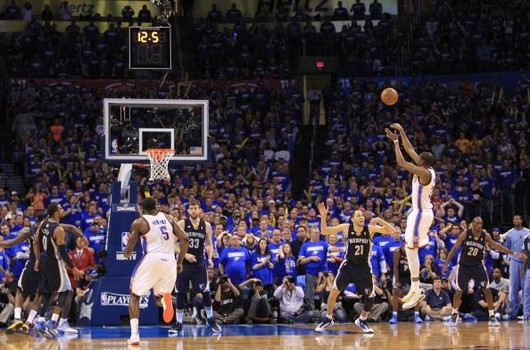
\includegraphics[width = 0.4\textwidth]{img/Triple.jpg}
\end{center}
\end{problem}

\begin{problem} Considera el $K$-homomorfismo $\appl{φ}{K[x,y]}{K[t]}$ con $φ(x) = t^2$ y $φ(t) = t^3$. Decide de manera razonada si φ factoriza por $\quot{K[x,y]}{\gen{x^2-y^2}}$. ¿Y por $\quot{K[x,y]}{\gen{x^3-y^2}}$?

\solution

\doneby{Guille}

Según se definía en la \fref{prop:FactorizacionHomomorfismo}, φ factoriza por $\quot{R}{I}$ si $I ⊂ \ker φ$, donde $\ker φ = \set{a ∈ R \tq φ(a) = 0}$. En el caso concreto de este ejercicio, lo que tenemos que ver es si $\gen{x^2 - y^2}$ y $\gen{x^3-y^2}$ están dentro de $\ker φ$.

Si $p(x,y) ∈ \gen{x^2-y^2}$, entonces $p(x,y) = a·(x^2-y^2)^n$ para $a ∈ K[x,y]$ y $n ∈ ℕ$. Calculando su imagen por $φ$, tenemos que \[ φ(p) = φ(a) · \left(φ(x^2) - φ(y^2)\right)^n = φ(a) · (t^4 - t^6)^n ≠ 0\], luego $\gen{x^2-y^2} \not\subset \ker φ$ y φ no factoriza por $\quot{K[x,y]}{\gen{x^2-y^2}}$.

Haciendo el proceso análogo con $p ∈ \quot{K[x,y]}{\gen{x^3-y^2}}$, nos saldrá que \[ φ(p) = φ(a) · (t^6 - t^6)^n = 0 \], así que $\gen{x^3-y^2} ⊂ \ker φ$ y $φ$ sí factoriza por $\quot{K[x,y]}{\gen{x^3s-y^2}}$.

\end{problem}

\begin{problem}[6] \textbf{Teorema chino del resto}. Sea $R$ un anillo y sean $I_1, \dotsc, I_n$ ideales en $A$. Consideramos el siguiente homomorfismo de anillos:
\begin{align*}
\appl{φ}{R&}{\quot{R}{I_1} × \dotsb \quot{R}{I_n}} \\
r &\longmapsto (r_1, \dotsc, r_n)
\end{align*} donde $r_i$ denota la clase de $r$ módulo $I_i$. Demuestra que:

\ppart φ es sobreyectiva si y sólo si $I_i$ e $I_j$ son primos entre sí cuando $i ≠ j$.
\ppart φ es inyectiva si y sólo si $\bigcap I_i = \zerogen$.

\textit{Sugerencia general: Empieza considerando el caso $n = 2$. Para el primer apartado, en $\implies$ hay que observar que $(1,0)$ y $(0,1)$ tienen preimagen; para $\impliedby$ basta comprobar que $(1,0)$ y $(0,1)$ tienen preimagen. Para el segundo apartado, calcula $\ker φ$.}

\solution

\doneby{Guille}

Recordamos que dos ideales $I,J ⊂ R$ son \concept[Ideal\IS coprimo]{Ideales\IS coprimos} si $I + J = R$.

\spart

Demostrarmos primero la implicación a la derecha: si φ es sobreyectiva, entonces $I_i$ e $I_j$ son primos entre sí cuando $i ≠ j$. Vamos a demostrar que cualquier $a ∈ R$, con $a ∉ I_i, I_j$ se puede expresar como suma de elementos de $I_i$ e $I_j$.

Consideramos la imagen de $a$, $φ(a) = (a_1, \dotsc, a_n)$. Como $a$ no está ni en $I_i$ ni en $I_j$, tiene que ser $a_i, a_j ≠ 0$. Ahora bien, podemos descomponer $φ(a)$ como suma de tres elementos $φ(a) = α + a_i·1_i + a_j · 1_j$, donde $1_i$ es un vector nulo salvo por un $1$ en la coordenada $i$ y $α$ tiene las mismas coordenadas que $φ(a)$ salvo por la $i$-ésima y $j$-ésima, que son nulas.

Como φ es sobreyectiva, todos los sumandos tienen preimágenes. En concreto, la de $α$ está en $I_i ∩ I_j$, y las de $a_i · 1_i$ y $a_j · 1_j$ están en $I_j$ y en $I_i$ respectivamente. Por las propiedades de homomorfismo, la suma de esas preimágenes será igual a $a$, luego efectivamente cualquier $a ∉ I_i, I_j$ se puede expresar como suma de elementos de $I_i$ y $I_j$, por lo que $I_i$ e $I_j$ son primos entre sí.

Para la implicación al otro lado, suponemos que $I_i, I_j$ son coprimos cuando $i ≠ j$, y tratamos de demostrar que $φ$ es sobreyectiva. Como nos dice la sugerencia, nos basta con demostrar que $1_i$ tiene preimagen para $i = 1, \dotsc, n$, ya que sólo con eso podremos construir cualquier elemento en la imagen.

Si $φ(a) = 1_i$, significa que $a ∉ I_i$ pero $a ∈ I_j$ si $i ≠ j$. Si tal $a$ no existe, eso significa que cualquier elemento que esté en todos los $I_j$ con $i ≠ j$ está también en $I_i$. Luego $I_i ⊆ I_j$ para cualquier $j = 1, \dotsc, n$, contradicción porque entonces $I_j + I_j = I_j$ y no serían coprimos.

\spart

Sabemos que $a ∈ \ker φ \iff φ(a) = (0, \dotsc, 0)$, es decir, si y sólo si $a ∈ \bigcap I_i$. En otras palabras, $\ker φ = \bigcap I_i$, y efectivamente ya sabemos que φ es inyectiva si y sólo si $\ker φ = \zerogen$.

\end{problem}

\begin{problem} Demuestra que

\ppart Si $\gcd (n,m) = 1$ entonces $ℤ_{n·m} \simeq ℤ_n × ℤ_m$.
\ppart Demuestra que $\quot{ℝ[x]}{\gen{(x^2-1)x^3}}$ es isomorfo a la suma directa de tres anillos locales, que dos de ellos son un cuerpo y que el tercero tiene nilpotentes.

\solution

\end{problem}

\begin{problem} Encuentra ejemplos de anillos que verifiquen las siguientes condiciones:

\ppart Un anillo que tenga exactamente 2 ideales maximales y al menos un nilpotente no nulo.
\ppart Un anillo con un único ideal primo \pideal (por tanto necesariamente maximal) que no sea un cuerpo.

\solution

\end{problem}

\begin{problem}[9] \label{ej:Hoja2:9} Demuestra que todo ideal $I \subsetneq R$ está contenido en un primo minimal siguiendo los siguientes pasos:

\begin{enumerate}
\item Considera el conjunto Σ de ideales primos de $R$ que contienen a $I$ y demuestra que no es vacío.
\item Define en Σ el siguiente orden parcial: $\mathfrak{p} ≤ \mathfrak{p}'$ si $\mathfrak{p}' ⊆ \mathfrak{p}$, y demuestra que toda cadena creciente de elementos en Σ tiene una cota superior en Σ.
\item Usa el \nref{lem:Zorn}.
\end{enumerate}

\solution

\spart


\end{problem}

\subsection{Problemas para entregar}

\begin{problem} Sea $R$ un anillo y sea $\mathfrak{p} ⊂ R$ un ideal primo. Demuestra que $\mathfrak{p}$ contiene un primo minimal, es decir, demuestra que existe un primo $\mathfrak{q} ⊂ \mathfrak{p}$ tal que si $\mathfrak{r} ⊂ R$ es otro ideal primo con $\mathfrak{r} ⊂ \mathfrak{q}$ entonces $\mathfrak{r} = \mathfrak{q}$.

\textup{Sugerencia: Puedes usar una idea parecida a la del \fref{ej:Hoja2:9}}.

\solution

\end{problem}


\begin{problem} Encuentra todos los primos minimales en $ℤ_{12}$,  $ℤ_9[x]$, $\quot{\K[x]}{\gen{x^3(x-1)}}$ y $\quot{ℝ[x,y]}{\gen{x-y^2}}$.

\solution

\end{problem}

\begin{problem} Sea $\appl{f}{R}{T}$ un homomorfismo de anillos.

\ppart Demuestra que si $J ⊂ T$ es un ideal entonces $\inv{f}(J) = \set{r ∈ R \tq f(r) ∈ J}$ es un ideal en $ℝ$. Demuestra que necesariamente $\ker f  ⊂ \inv{f}(J)$.
\ppart Demuestra que si $I ⊂ R$ es un ideal, entonces $f(I) = \set{f(r) \tq r ∈ I}$ en general no es un ideal en $T$.
\ppart Demuestra que si $I ⊂ R$ es un ideal y $f$ es sobreyectiva entonces $f(I)$ es un ideal en $T$.

\ppart Sea $I ⊂ R$ un ideal. Aunque en general $f(I)$ no tiene por qué ser un ideal en $T$, podemos considerar el ideal que genera en $T$. Denotaremos por $I^e$ al ideal generado por $f(I)$ en $T$.  Demuestra que $I ⊂ \inv{f}(I^e)$ y que en general el contenido es estricto.
\ppart Sea $J ⊂ T$ un ideal. Demuestra que $(\inv{f}(J))^e ⊂ J$ y que en general el contenido es estricto.

\solution

\end{problem}

\begin{problem} Trabajamos en $ℝ[x,y]$. Sean $a,b ∈ ℝ$. ¿Cuál es la condición necesaria y suficiente para que un maximal de la forma $\gen{x-a, y-b}$ contenga al ideal $\gen{x-y^2}$?


\textup{Sugerencia: $\gen{x-y^2} ⊂ \gen{x-a, y-b}$ si y sólo si el homomorfismo del paso al cociente $ℝ[x,y] \mapsto \quot{ℝ[x,y]}{\gen{x-a, y-b}} \simeq ℝ$ factoriza por $\quot{ℝ[x,y]}{\gen{x-y^2}}$. ¿Por qué? Y ahora piensa, ¿cuál es el homomorfismo composición $ℝ[x,y] \mapsto ℝ$?}

\solution

\end{problem}


\begin{problem} Demuestra que el ideal $\gen{x^2 + x - y} ⊂ ℝ[x,y]$ es primo. ¿Es maximal?

\solution

\end{problem}

